%last\documentclass[aps,pre,showpacs,amsmath,amsfonts,amssymb,superscriptaddress,twocolumn,floatfix]{revtex4-1} 
\documentclass[aps,pre,showpacs,twocolumn,superscriptaddress,floatfix]{revtex4-1}
%\documentclass[aps,pre,showpacs,onecolumn,superscriptaddress,floatfix]{revtex4}
\usepackage{graphicx}
%\usepackage{epsfig} 
%\usepackage{epstopdf}
\usepackage{color}
\usepackage{amsfonts}
\usepackage{amssymb,amsmath}
\usepackage{grffile}
\usepackage{pgfplots}
\usepackage{hyperref}
\usepackage{amsmath}
% \usepackage[backend=biber]{biblatex} 

\usepackage{todonotes}
\usepackage{color}

\newcommand{\Ham}{\mathcal{H}}
\newcommand{\Ntilde}{\widetilde{N}}
 
\begin{document}

\title{Thermal relaxation and heat transport in one-dimensional systems: a comparative study}
 
\author{Carlos Olivares}
\affiliation{Department of Physics, PUC-Rio, Rio de Janeiro, Brazil}

\author{Celia Anteneodo}
\affiliation{Department of Physics, PUC-Rio, Rio de Janeiro, Brazil} 
%\affiliation{Institute of Science and Technology for Complex Systems, Rio de Janeiro, Brazil}


\date{\today}

\begin{abstract} 
By means of molecular dynamics simulations, we analyze the relaxation to equilibrium 
of one-dimensional systems, after applying a kinetic energy perturbation. 
We consider systems of rotators, linear and nonlinear oscillators. 
The relaxation time $\tau$ follows a scaling with size $N$, $\tau \sim N^\delta$, where $\delta$ 
depends on the kind of system and energy range. 
We relate this result with the scaling of the conductivity $\kappa \sim N^\gamma$ and discuss 
this relation with the type of heat diffusion. 
%We that show that, under this protocol,  short-range systems exhibit a slower relaxation 
%that the long-range ones. We also compare these results to the outcomes for short-range 
%linear and nonlinear oscillators. 
\end{abstract}

\pacs{
44.10.+i,  %Heat conduction 
05.60.-k,   % Transport processes
05.70.Ln,  %Nonequilibrium and irreversible thermodynamics 
%65  thermal properties of condensed matter
66.30.Xj	%Thermal diffusivity
}
\maketitle

 
%%%%%%%%%%%%%%%%%%%%%%%%%%%%%%%%%%%%%% 

\section{Introduction}

 
% It is well know that the ergodicity
The study of the relaxation of a system towards equilibrium is important   
to understand the nature of irreversibility and   
non-equilibrium properties of a system
\cite{Kardar2007statistical,Huang1987statistical,Kubo1992statistical,Gallavotti2008BoltzmannLegacy}. 
In particular, heat conduction.
%However, until today remains open questions in the fundamental basis
%of statistical mechanics, like a rigorous proof 
%of the ergodicity problem which establish 
%the relation between kinetic approach and the ensemble 
%theory \cite{Livi1985PRA,Jin2013EquiTherma} 
%, by the assumption that the time average is equivalent to the ensemble average, 
%or the difficulties of use Gibbs statistical mechanics
%for long-range interacting systems 
%in which new phenomena emerge such as ensemble inequivalence,
%negative specific heat and phase transitions for one dimensional 
%systems \cite{CampaDauxoisRuffo2009PhysRep}.
%
%Nonetheless, statistical physics of systems for 
%short-range systems give us a good understanding 
%of physical systems in equilibrium. In spite of that,
%real equilibrium systems is almost never achieve in nature
%where almost every systems is out of equilibrium.
%
Even with the enormous efforts to understand non-equilibrium phenomena
a general theory is still lacking~\cite{ReviewDhar2008,ReviewLepriLiviPoliti2003}. 
%
Numerical simulations provide an alternative approach, allowing the realization of 
computer experiments. For instance, by applying reservoirs at different
temperatures to a system, or preparing an isolated system  with a 
non-uniform temperature and let it evolve to the equilibrium 
\cite{ReviewBonettoLebowitzReyBellet2000}.
A connection between these two approaches is possible,
for instance, if the Fourier law is satisfied. 
In such case, the conductivity must be inversely proportional to
the relaxation time of an out-of-equilibrium system~\cite{Lampin2013}.
Notwithstanding, Fourier's law is not always satisfied in one-dimensional
systems~\cite{ReviewDhar2008,ReviewLepriLiviPoliti2003,OlivaresAnteneodo2016PRE} and can  present
anomalous transport ($\kappa \sim N^a$)~\cite{ProsenCampbell2000PRL}. 
% or apparently another non-conserve quantity \cite{DasDhar2015}. %% FIXME:
%

Therefore, the investigation of the connection between relaxation and
the thermal conductivity is a relevant issue, that can contribute both 
to the fundamental basis \cite{Lepri1998PRE,GendelmanSavin2010PRE}, as well 
as to practical   applications \cite{ZaouiPallaCleriLampin2016PRB,Lampin2013}.

% a general definition of relaxation times in Hamiltonian systems 
% remains an open question \cite{Maiocchi2010,Piazza2001}.

On the other hand, long-range systems introduce additional difficulties, 
such as  ensemble inequivalence \cite{BarreMukamelRuffo2001PRL}. 
The relaxation times in long-range systems
are typically larger than in short-range ones
\cite{MukamelRuffoSchreiber2005,Miloshevich2015PRE,AntunesLevin2015PRE,
BagchiTsallis2017,Teles2015PRE}. 
%

Motivated by recent works on thermal transport 
\cite{Bagchi2017PRE,OlivaresAnteneodo2016PRE,Pereira2013PRE}, 
we explore the relaxation times of systems when
a system  is subjected to large thermal perturbations.

In this paper we consider for four different systems, namely,...  
when is applied a temperature
split protocol with periodic boundary conditions ($q_{N+1}= q_1$). 

 
%%%%%%%%%%%%%%%%%%%%%%%%%%%%%%%%%%%%%% 
\section{Systems and Methods} 
\label{sec:ModelMethods}


We consider one-dimensional model systems, 
governed by a classical Hamiltonian of the general form
%
\begin{equation}
 \Ham =\frac{1}{2} \sum_{i=1}^{N} p^2_i +  \mathcal{U}(q_1,\ldots,q_N)  \,.
\end{equation}
%
yielding the equations of motion:

\begin{equation}
\begin{split}
 \dot{q}_i & = p_i, \hspace{1cm} \text{ for } 1 \le i \le N, \\
 \dot{p}_i      & = -\frac{\partial \mathcal{U}}{\partial q_{i} } \,.
\end{split}
\label{eqmotion}
\end{equation}
Boundary conditions are periodic. 
We will  analyze as particular cases   rotators 
 with ferromagnetic-like (either short and long range) couplings, linear oscillators, and  
 non-linear Fermi-Pasta-Ulam-Tsingou springs, as described below. 
%
 
 

We consider the $\alpha-XY$ classical rotators~\cite{Anteneodo1998,TamaritAnteneodo2000}, 
a paradigmatic model that allows to control the range of the interactions,  whose 
potential energy is defined as  


\begin{equation}
  \mathcal{U}  =
  \frac{1}{2 \widetilde{N}^\alpha}  \sum_{i=1}^N  \sum_{j \neq i}^N   
	\frac{\mathcal{V} (q_i - q_j)}{r_{i,j}^\alpha} \,,
\label{Halfa}
\end{equation}
%
where 
%
\begin{equation}
\mathcal{V}(x)=1-\cos x \,,  
\end{equation}
%
$r_{i,j}$ is the minimal distance 
between rotators $i$ and $j$, over the circle of length $N$, and the normalization factor is   
\begin{equation}
 \widetilde{N}^\alpha \equiv 2 \sum_{r=1}^{N/2} r^{-\alpha} = %
 \begin{cases}
   2 &\text{if $\alpha \to \infty$}, \\
   N &\text{if $\alpha = 0$}.
 \end{cases}
\end{equation}
%
We will focus in these extreme cases, that correspond to pairwise nearest-neighbor ($\alpha\to\infty$) 
and global ($\alpha=0$) couplings. 
% 
In the first case, the total potential  energy becomes
%
\begin{equation}
  \mathcal{U}  = \frac{1}{2} \sum_{i=1}^N   \mathcal{V}(q_i - q_{i+1})  \,.
\label{Hshort}
\end{equation}
%
In the latter case, also known in the literature as HMF~\cite{AntoniRuffo1995PRE}, 
the total potential energy takes the form
%
 \begin{equation}
  \mathcal{U}  =
  \frac{1}{2  N}  \sum_{i=1}^N  \sum_{j \neq i}^N {\mathcal{V}(q_i - q_j)} \,.
\label{Hlong}
\end{equation}
 
  
We will also investigate the following simple short 
range systems, where the interaction energy in Eq.~(\ref{Hshort}) is given by 
%   
\begin{equation}
 \mathcal{V}(x) = 
 \begin{cases}
  \frac{x^2}{2}  &\text{(HC),} \\[2mm]
  \frac{x^2}{2}+ \frac{x^4}{24}  &\text{($\beta$-FPUT),}  
 \end{cases}
 \label{eq:Potentials}
\end{equation}
%
corresponding to  chains of harmonic (HC) and  an-harmonic Fermi-Pasta-Ulam-Tsingou   springs
($\beta$-FPUT, with $\beta=1/6$)~\cite{BermanIzrailev2005Report,Dauxois2008PhysToday}.
%

	
Numerical integration of the equations of motion (\ref{eqmotion}) was 
performed by means of a fourth-order symplectic algorithm~\cite{Yoshida1990}, 
 with periodic boundary conditions. 
%
As initial condition, we set $q_i = 0$ for all $i$ so that all the energy is purely kinetic ($E=K$), 
and draw the $p_i$, $i=1,\ldots,N$  from a uniform distribution. Then, the 
velocities were shifted, to make the total momentum zero, and scaled 
to obtain the desired total energy $E=K=N T/2$, where $T=\sum_i^N p_i^2/N$ is the temperature. 
%
For each realization, we waited until the isolated system attained equilibrium, 
identified by the theoretical equilibrium value of the partition between potential and kinetic energies, 
as well as by  the Maxwellian distribution of velocities. 
 
Once at equilibrium, the following perturbation was applied, at a time $t=0$: 
%  
we perturbed the system through a kinetic energy split protocol, 
without affecting the coordinates $q_i$, and keeping  the total energy of the system unchanged. 
The split protocol consists in defining two subsystems $S_h$ (hot) and $S_c$ (cold),  
 in our case composed by the particles $i=1,2,\dots, N/2$ and $ N/2+1, \dots, N$, respectively.
% 
The velocities of $S_c$ are set to zero, while the velocities of $S_h$ are scaled by a factor $2T$, 
in order to exactly compensate the kinetic loss of $S_c$, after a correction to guarantee zero 
total momentum. 
%
Then,  we monitored  the relaxation energies of each subsystem, 
keeping the whole system isolated at the initial total energy $E$. 
In all cases we measured average energies over $2^{18}/N$ realizations. 
%
Characteristic equilibration times were computed for   different sizes $N$ and 
 energies per particle  $ u=E/N $.




	
\section{Relaxation behavior}

\subsection{Short-range XY rotators}
\label{sec:short}


Let us start by analyzing the short-range XY model,  identified  by Eq.~(\ref{Hshort}). 
This is an exceptional model in the scenario of thermal transport since it 
is a momentum conserving system with normal 
heat transport, i.e. finite thermal conductivity 
\cite{GiardinaLiviPolitiVassali2000PRL,GendelmanSavin2000PRL,
ReviewLepriLiviPoliti2003,ReviewDhar2008,OlivaresAnteneodo2016PRE}.
%
This behavior is attributed to the non-conservation of
stretch or the presence of phases (finite and periodic potential energy)~\cite{DasDhar2015}. 

\begin{figure}[h!]
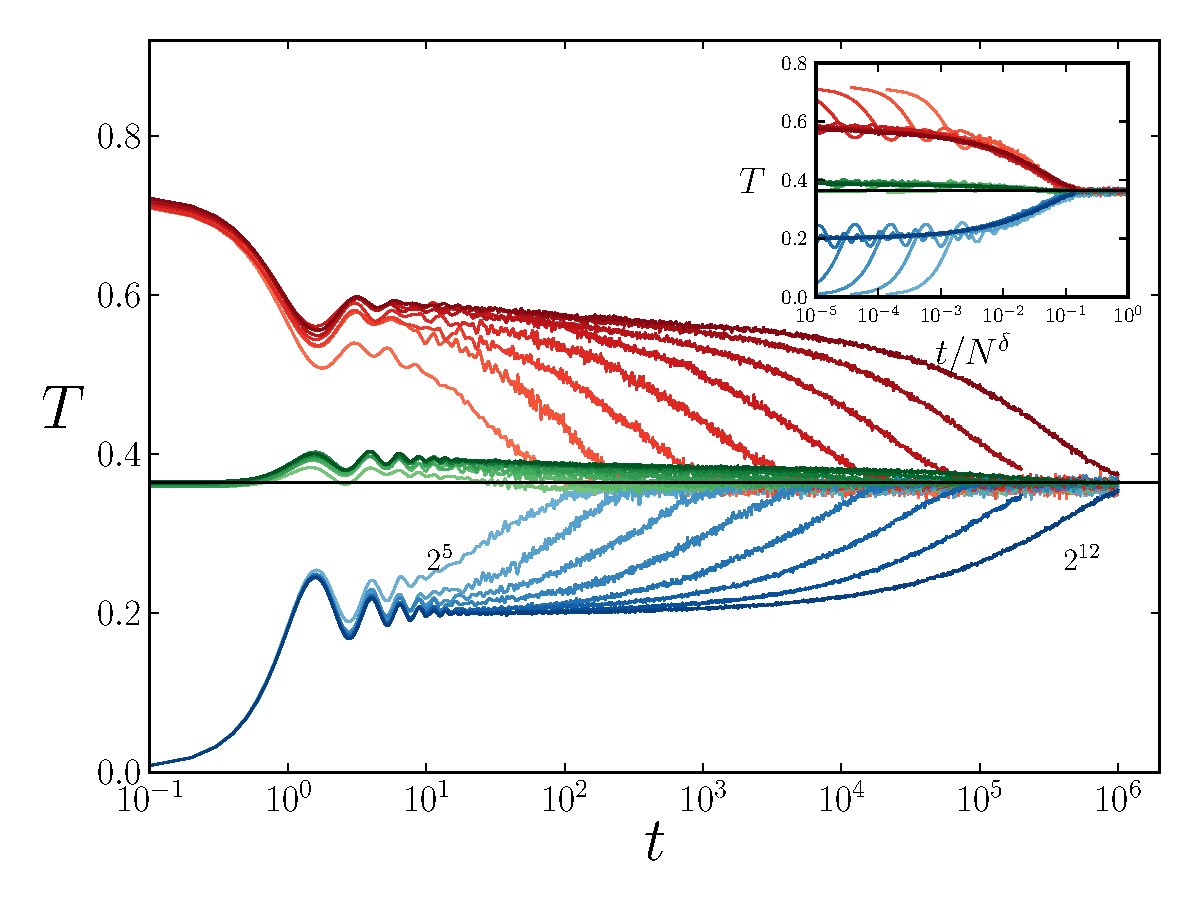
\includegraphics[width=1.0\linewidth]{TempLogt_XY__U_0.4__Delta_1.9.pdf}
\caption{Nearest-neighbor XY rotors: relaxation towards equilibrium, for $u=0.4$. 
Temperature of hot (red), cold (blue) subsystems, and whole system (green) 
versus time  $t$,   averaged  over $2^{13}/N$ realizations.  
System sizes range  are $N=2^k$, $k=5, \ldots, 12$.
%
The black horizontal line represents the theoretical equilibrium value. 
Inset:  temperatures versus scaled time $t/N^\delta$, where $\delta=1.9$ was used. 
 }
\label{fig:nn04}
\end{figure}

\begin{figure}[h!]
 \centering
 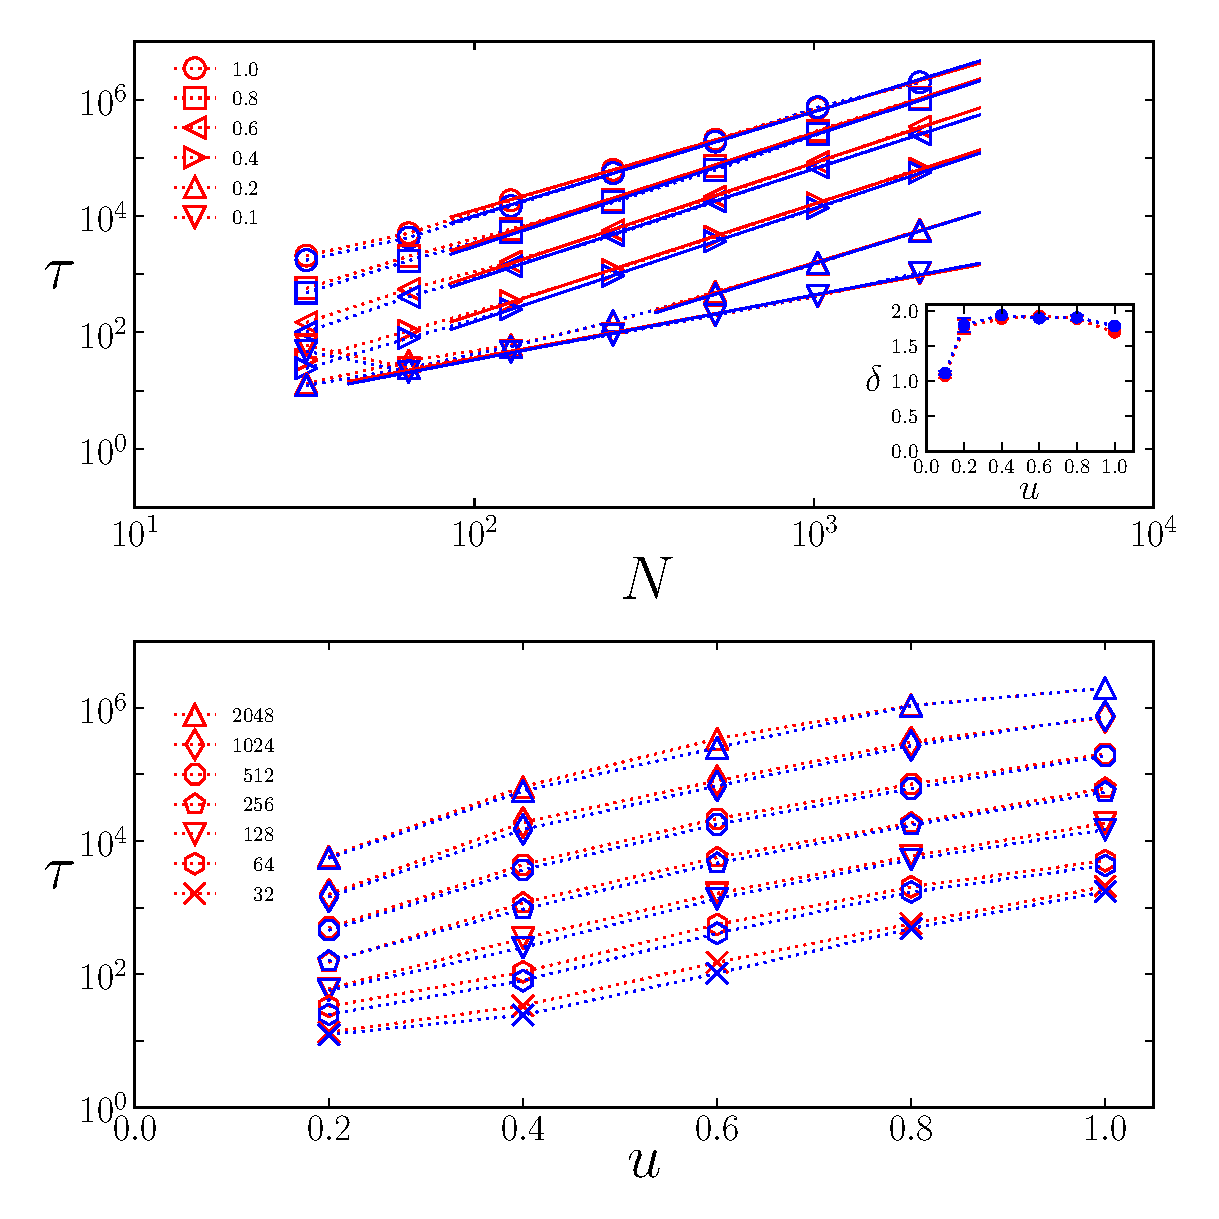
\includegraphics[width=1.0\linewidth]{./Taus1over5_XY.pdf}
 \caption{Nearest-neighbor XY rotors: 
(a) Relaxation time $\tau$ versus  system size $N$
 for different values of energy $u$. 
The solid lines correspond to a power-law fitting with exponents shown in the inset. 
(b) Relaxation time $\tau$ versus  $u$ for different values of $N$. 
Results for hot and cold subsystems are shown by red and blue symbols respectively.  
}
 \label{fig:Taus1over5_XY}
\end{figure}

A representative relaxation portrait after the split protocol is shown in Fig.~\ref{fig:nn04},  
for energy density $u=0.4$ and several systems sizes. 
We represent the (averaged) temperature of each subsystem as well as the temperature of the whole system. 
%and scaling exponent $\delta=1.77$.
%

We notice an initial regime of violent relaxation with small oscillations, 
almost insensitive to system size, followed by a  regime of longer duration, 
that strongly depends on system size. 
%
%We notice a slight asymmetry between the relaxation of hot and cold subsystems, 
%that increases with energy.
% and decays with time.????
%
The decay is nearly exponential but instead of obtaining exponential rates 
from a fitting procedure, we estimated the relaxation time,  $\tau_s$, for $s=h,c$   
as the time interval required for the temperature difference 
$\Delta T_s(t) \equiv T_s(t) - T_{eq}$,  
to fall  to 20\% of its equilibrium value, $T_{eq}$,   
that is 
%
%\begin{equation}
 $\Delta T_s(\tau_s)       = 0.2 \Delta T_s(0)$.
%\label{eq:RelaxTimeDef}
%\end{equation}

 
The behavior of the relaxation time $\tau$ versus $N$ 
  is presented in Fig.~\ref{fig:Taus1over5_XY}(a). 
%
We observe a scaling behavior  $N^\delta$, with values of $\delta$ shown in the inset. 
These values are slightly below 2 for sufficiently large energies per particle $u$ but become close to 1 for 
 $u \lesssim 0.1$. 
%
Moreover, $\tau$ increases with $u$, almost exponentially, as shown in Fig.~\ref{fig:Taus1over5_XY}(b).
%??? talvez nao mostrar painel inferior  


\begin{figure}[h!]
 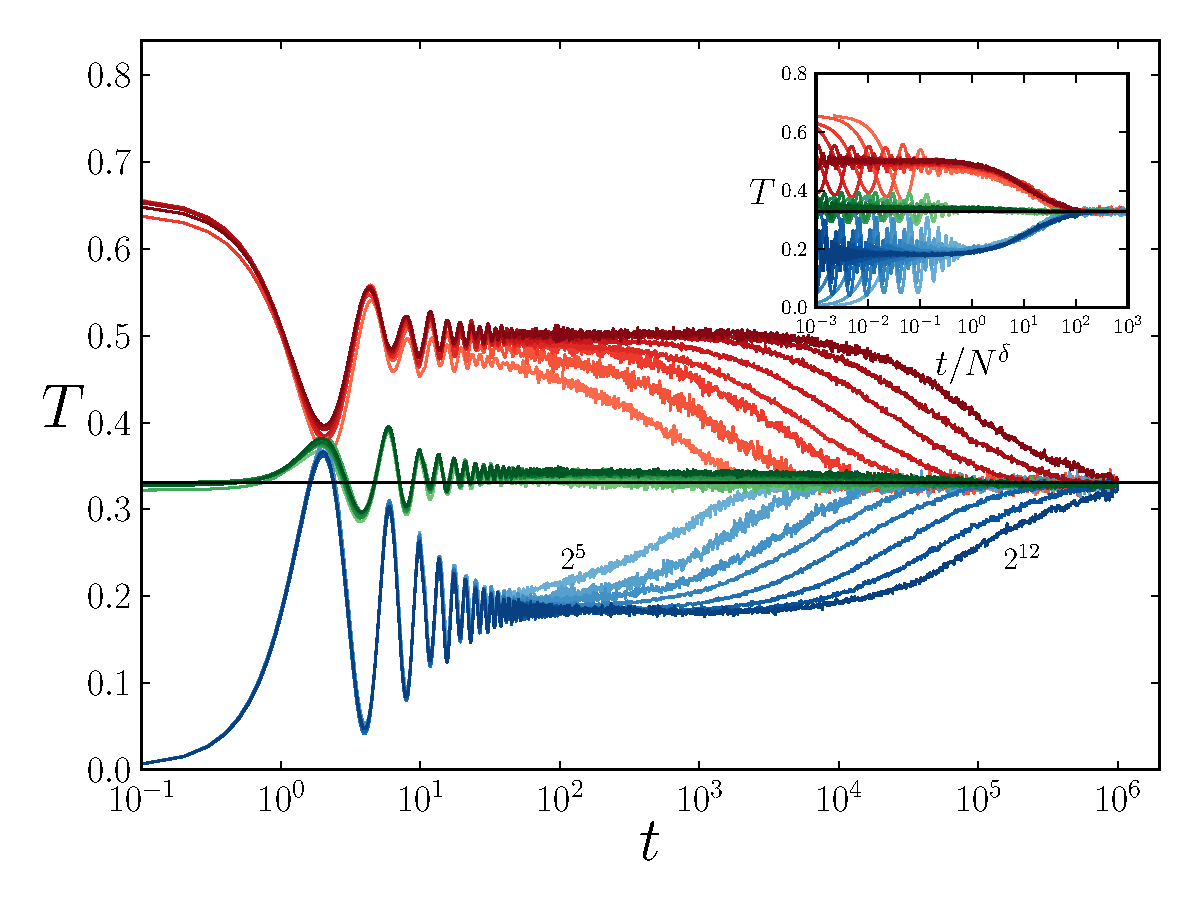
\includegraphics[width=0.95\linewidth]{TempLogt_HMF__U_0.4__Delta_1.09.pdf}
 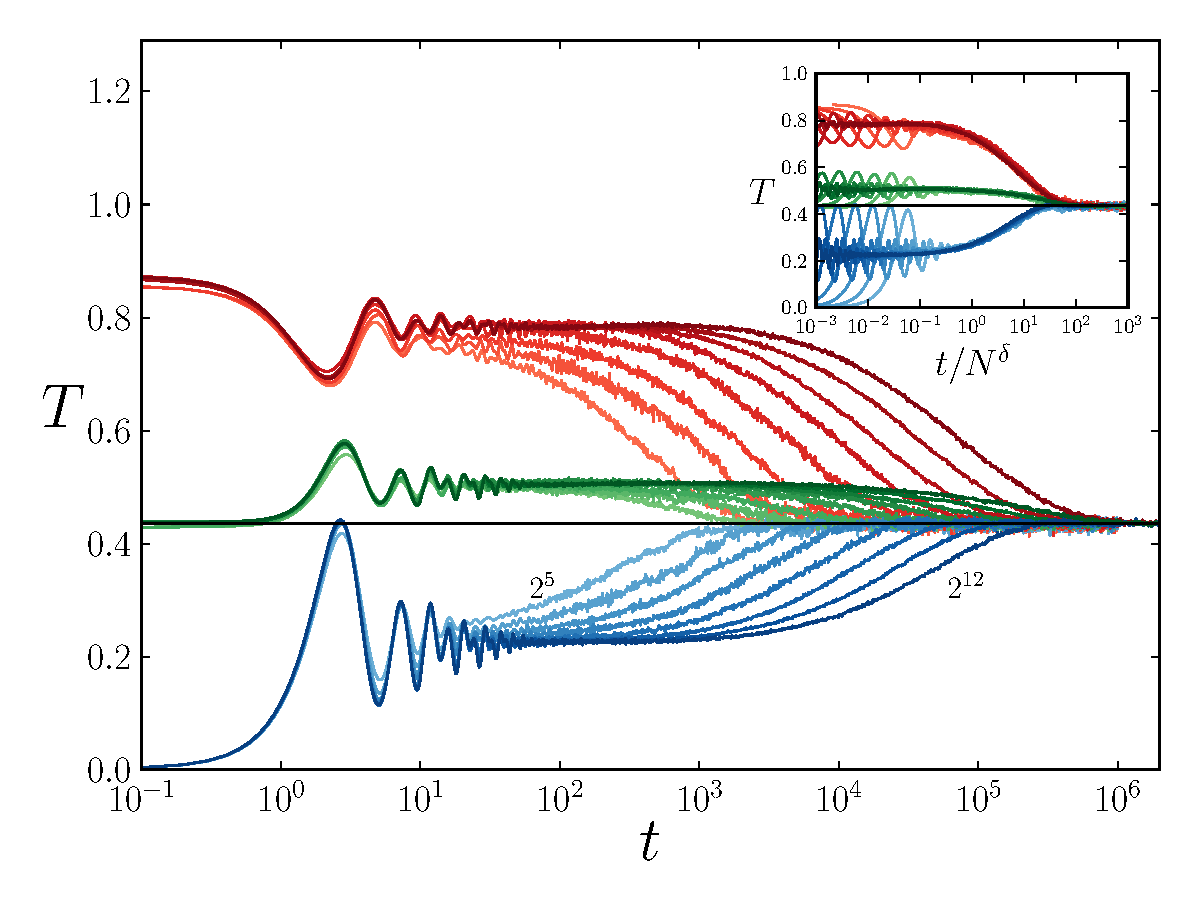
\includegraphics[width=0.95\linewidth]{TempLogt_HMF__U_0.6__Delta_1.11.pdf}
%
\caption{Mean-field XY rotators: relaxation towards equilibrium for $u=0.4$ (a) and $u=0.6$ (b). 
Temperature of hot (red), cold (blue) subsystems, and  whole system (green) versus  time $t$.  
System sizes are $N=2^k$, $k=5, \ldots, 12$. 
The black horizontal line represents the theoretical equilibrium value. 
Insets: temperatures versus  scaled time $t/N^\delta$, where $\delta=1.09$ (a) and $1.11$ (b). 
}
\label{fig:mf06}
\end{figure}

%%%%%%%%%%%%%%%%%%%%%%%%%%%%%%%%%%%%%%%%%%%%%%%%%%%%%%%%%%%%%%%%%%%%%%%%%%%%%%%%%%%%%%%%
\subsection{Long-range XY rotators}
\label{sec:long}




Now we address  the HMF model, identified  by Eq.~(\ref{Hlong}).  
%
The relaxation of temperatures are shown in Fig.\ref{fig:mf06}. 
Like in the short-range case, we observe a first regime that is independent of system size but 
with larger oscillations in this long-range case, followed by a size-dependent decay. 
For $u=0.4$, Fig.\ref{fig:mf06}(a), the profiles are nearly symmetric. 
For $u=0.6$, Fig.\ref{fig:mf06}(b), there is a noticeable asymmetry and a delay of the cold subsystem 
with respect to the hot one. These effects are less pronounced at $u=0.4$ and in the short-range case. 




It is worth mentioning, that even if the temperature attained the theoretical equilibrium 
value, the velocity probability distribution becomes Gaussian at later times, as depicted in 
Fig.~\ref{fig:Kurt_HMF}, were we plotted the kurtosis versus time.   
Differently, in the short range case the Gaussian distribution is attained concomitantly with 
the equilibrium value of the temperature. 


\begin{figure}[h]
 \centering
 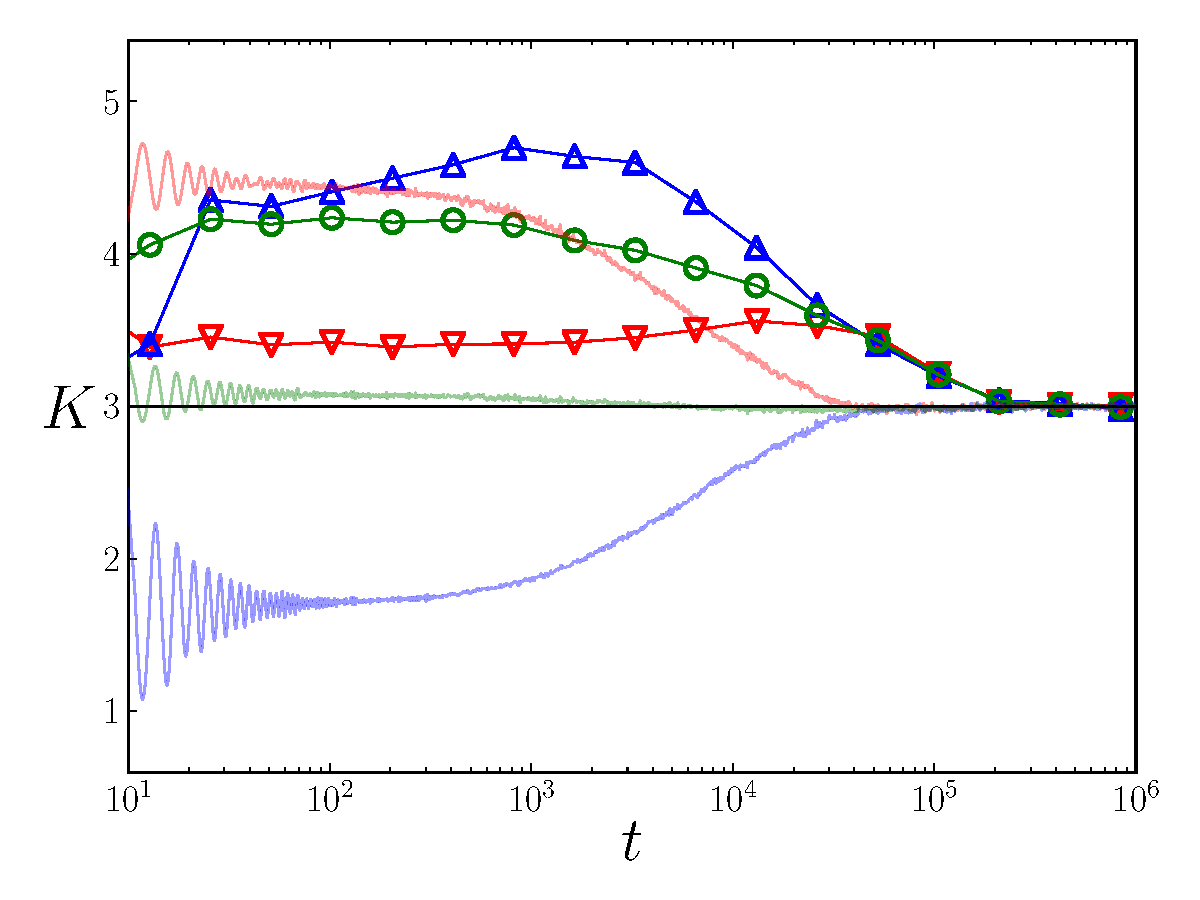
\includegraphics[width=0.95\linewidth]{./Kurt_HMF__U_0.4__N_256.pdf}
 % Kurt_HMF__U_0.4__N_256.pdf: 576x288 pixel, 72dpi, 20.32x10.16 cm, bb=0 0 576 288
 \caption{Temporal evolution of the kurtosis of the velocity distribution of mean-field XY 
 rotators, for $N=256$ and $u=0.4$. 
The solid line corresponds to the Gaussian value   $k_4=3$, drawn for comparison.
}
 \label{fig:Kurt_HMF}
\end{figure}



The behavior of the relaxation time versus $N$ is presented in Fig.~\ref{fig:Taus1over5_HMF}(a)-(b). 
The relaxation time increases with $N$ following approximately the scaling behavior $\tau \sim N$. 
%
Furthermore,   the symmetry of the profiles observed for small energies [e.g. $u=0.4$ in Fig.~\ref{fig:mf06}(a)] 
is reflected in nearly coincident relaxation times. 
However,  for higher energies, the asymmetry  [e.g. $u=0.6$ in Fig.~\ref{fig:mf06}(b)] 
is related to the shorter relaxation times of the cold subsystems.  


%
The dependency of $\tau$ on the energy is depicted in  Fig.~\ref{fig:Taus1over5_HMF}(c) 
for two different system sizes. 
In contrast to the short-range case, $\tau$ does not increase monotonically with $u$, but presents 
a minimum value near the critical energy ($u=0.75$) at which a continuous ferromagnetic transition 
occurs~\cite{Anteneodo1998}. In this region there is also 
enhanced dependency on the system size. 
 
 
\begin{figure}
 \centering
 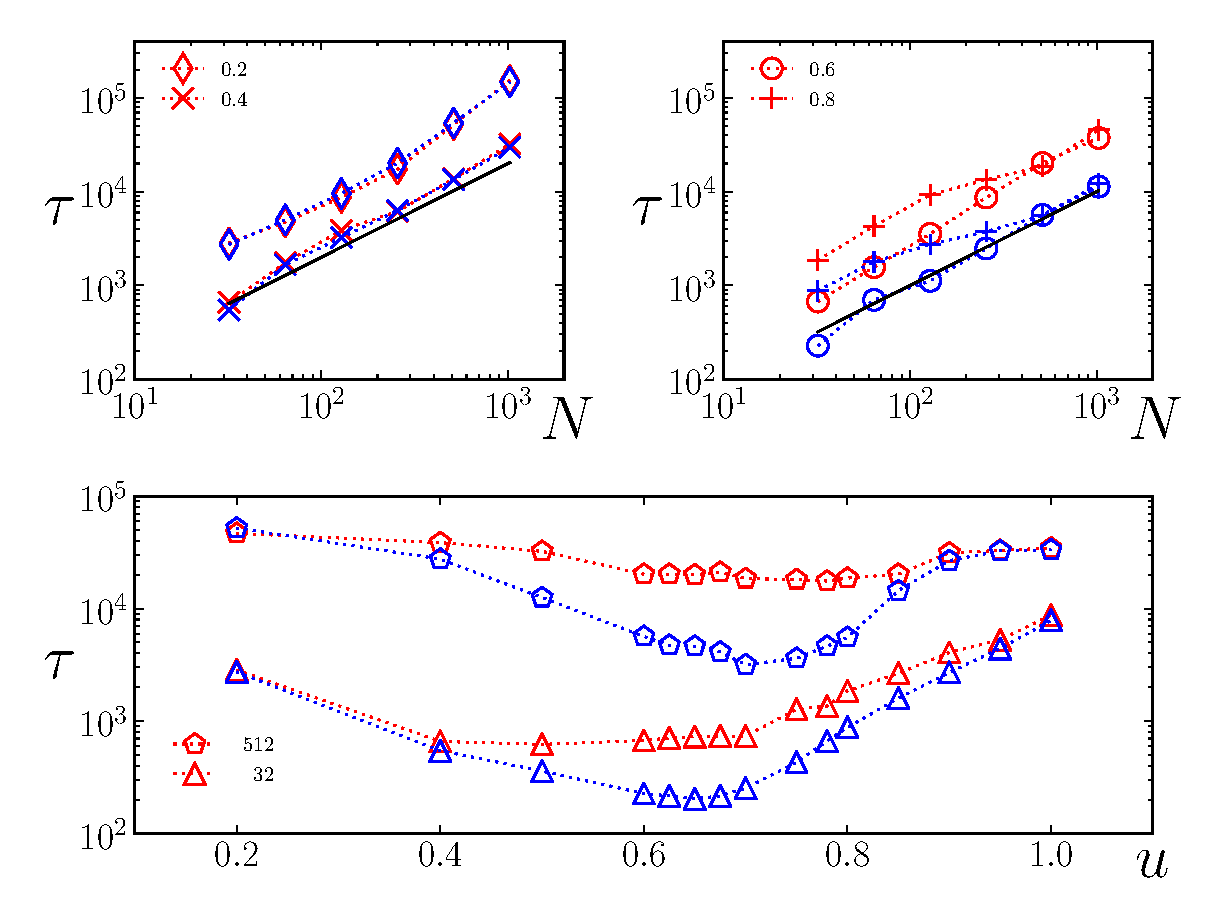
\includegraphics[width=0.95\linewidth]{./Taus1over5_HMF_final.pdf}
 \caption{Mean-field XY rotators:  relaxation time $\tau$ as a function of  system size $N$
 for different values of energy $u$ (a)-(b). 
The solid lines have slope 1, drawn for comparison. 
%
Relaxation time as a function of  $u$, for two different system sizes (c). 
Results for the hot and cold subsystems are shown by red and blue symbols respectively. 
In all cases averages over $2^{18}/N$ realizations are shown.  
}
 \label{fig:Taus1over5_HMF}
\end{figure}

%%%%%%%%%%%%%%%%%%%%%%%%%%%%%%%%%%%%%%%%%%%%%%%%%%%%%%%%%%%%%%%%%%%%%%%%%%%%%%%%%%%%%%%%

\subsection{Oscillators}
\label{sec:other}

In order shed some light on the found scaling laws,  we investigate the linear 
and nonlinear oscillators given by Eq.~(\ref{eq:potentials}). 
 

%%there is not equipartition between the normal modes, 
%which are non interacting. Therefore, the initially excited modes
%remain excited all the times. 
%However, the partition  between the average kinetic and potential energies must satisfy
%the virial theorem, such that  we get  $T= \sum_i^N p_i^2/N=u$.

In the purely harmonic case, the temporal evolution of $T$ is shown 
in Fig. \ref{fig:TempLogt_HC__U_0.4} 
for $u=0.4$ and different system sizes.   
%
Despite the noisy profiles, probably related to the lack of interaction between modes, 
the scaling behavior is neatly $\tau \propto N$, that is, $\delta=1$. 
%
Moreover, we observed that this scaling exponent  is energy independent, differently to the 
previous cases.
%

This scaling law explains the change of behavior observed in the plots of $\tau$ versus $N$, 
in the short-range XY case at low energy (see Fig.~\ref{fig:Taus1over5_XY}). 
In fact, at low energies, the rotors feel the nearly harmonic bottom
of the potential well, reaching the limit of harmonic oscillators.



\begin{figure}[h]
 \centering
 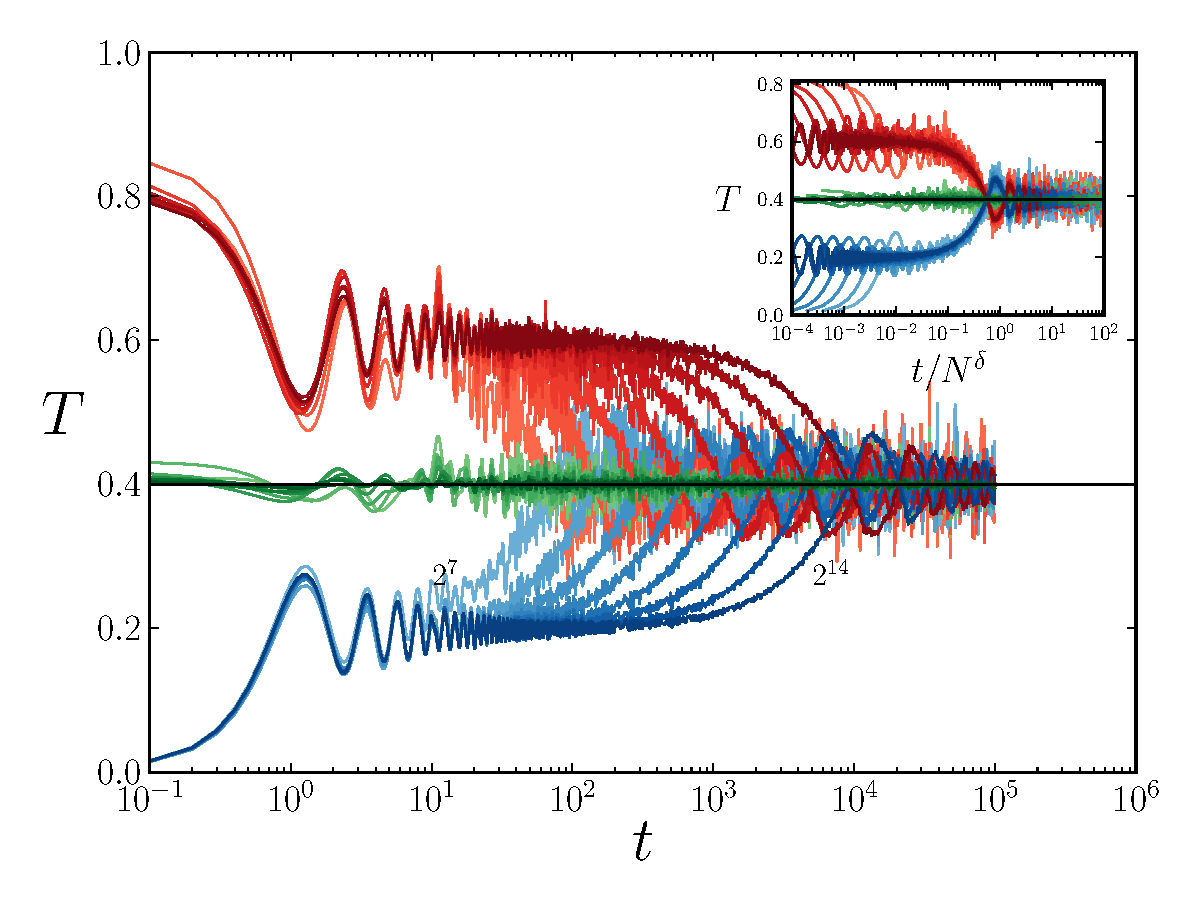
\includegraphics[width=1.0\linewidth]{TempLogt_HC__U_0.4__delta_1.0.pdf}
 % TempLogt_HC__U_0.4.pdf: 585x441 pixel, 72dpi, 20.64x15.56 cm, bb=0 0 585 441
 \caption{Harmonic chain: relaxation to equilibrium, as in previous figures, 
 with $u=0.4$, for sizes $N=2^{k}$ for $k=7 \ldots, 14$. 
 The inset  shows the scaled data, with $\delta = 1$. 
}
 \label{fig:TempLogt_HC__U_0.4}
\end{figure}


Finally, we investigate the effect of nonlinearities, such as those introduced 
by the  $\beta$-FPUT interaction potential, 
largely studied over the past 60 years ~\cite{BermanIzrailev2005Report,Dauxois2008PhysToday}. 
% shown an unexpected recurrence when the first normal mode was excited 
%and no equipartition between the modes was achieved. However, this 
%no equipartition problem is due to the weak chaotic regimen 
%that the FPUT was under the excitation of the first mode in the original 
%problem \cite{Pettini2005Chaos}.
{


In Fig. \ref{fig:TempLogt_FPU__U}, we show  representative   
equilibration profiles for  the $\beta$-FPUT, 
of different sizes.
%
We found a time scaling factor $t/N^\delta$, where $\delta \simeq 1.68 $ 
for $u =0.4$ (see inset Fig. \ref{fig:TempLogt_FPU__U} ).
%
This value of $\delta$ was obtained by fitting the exponential law 
$\Delta T_s(t) \sim \exp(-t/\tau)$ at the final stages of equilibration,  
%
for sizes $N>1024$,  
when large oscillations around the equilibrium temperature are absent. 
%{\color{red} This oscillations have a different scale factor and have asymmetric
%amplitude also in the Fig. scale with $N$}
%
The time scale $t/N^\delta$ collapse is shown in the inset, for $\delta = 1.68$. 


\begin{figure}[h]
 \centering
 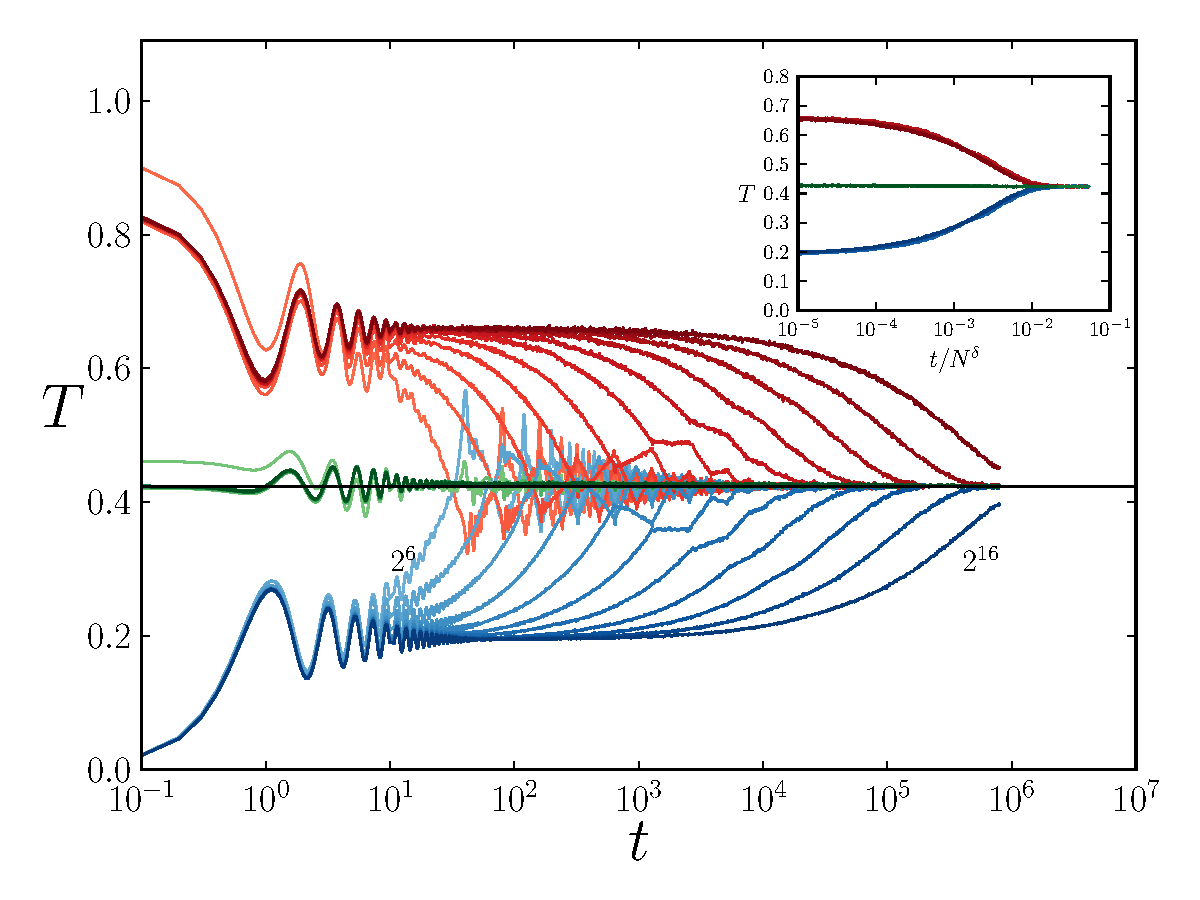
\includegraphics[width=1.0\linewidth]{TempLogt_FPU__U_0.4__Delta_1.68.pdf}
 \caption{FPUT oscillators with $\beta = 1/6$: relaxation to equilibrium, 
for $u=0.4$, and sizes $N=2^{k}$ for $k=6, \ldots 16$. 
%
The scaling collapse is shown in the inset, using $\delta = 1.68$ for $N>2^{13}$.
}
 \label{fig:TempLogt_FPU__U}
\end{figure}


In Fig.~\ref{fig:tau_FPU_HC}, we show the scaling behavior os the oscillator systems.

\begin{figure}[h]
 \centering
 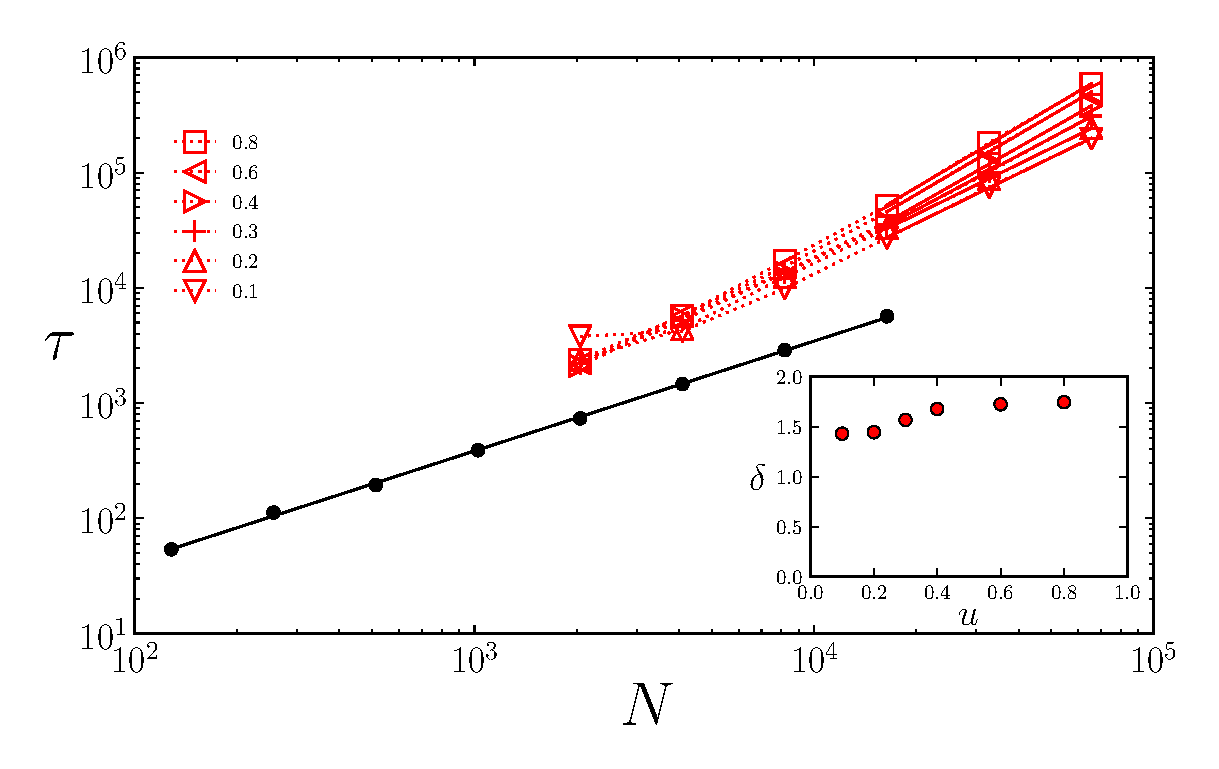
\includegraphics[width=1.0\linewidth]{./tau_FPU_HC.pdf}
 \caption{Oscillators: relaxation time $\tau$ versus $N$,  for different values of $u$. 
The small filled circles correspond to the chain of harmonic oscillators ($u=0.4$), 
the full line has slope $\delta=1$.
While the open symbols correspond to the FPUT chain at the energies indicated on the figures. 
The inset shows the scaling exponent for the FPUT systems as a function of $u$. 
}
 \label{fig:tau_FPU_HC}
\end{figure}




% \subsection{Other short range systems }







%%%%%%%%%%%%%%%%%%%%%%%%%%%%%%%%%%%%%% 
\section{Final comments}

In Fig.~\ref{fig:Taus_XY_HMF}, we present a comparison of the short and long-range XY systems, 
 showing that the relaxation is slower in the former case, with a larger scaling exponent, 
for the applied perturbation. 
While, for the long-range case the scaling is linear, $\tau \sim N$, 
for short-range rotators, the scaling is nearly $\tau \sim N^2$, at not too low energies, 
while also in this case the $\tau$ scaling is linear for very low energies. 
In fact, this  is the law observed for linear oscillators. 
Why long-range rotators behave as linear oscillators is not clear.....

In a recent work, Bagchi and Tsallis investigated a long-range version of the $\beta$-FPUT
\cite{BagchiTsallis2017}, finding a scaling $\tau \sim N^{1.8}$. 
Although the perturbation is different, the main source of discrepancy may come from the fact 
that the interaction between subsystems is short-range. Perhaps this is the reason 
why the scaling is closer to our short-range value, despite the subsystems are long-range. 

 
Moreover, in the long-range XY, at energies  near  the  phase 
transition critical value $u=0.75$, the relaxation times are asymmetric. 
%
The cold subsystem reaches equilibrium before the hot one for high energies. 
Moreover, even when  equilibrium  values have been attained in average, the distribution 
of velocities becomes Gaussian later.  

{\em 
Another contribution of this work is that even that the for the nearest neighbor rotators 
the system has a finite thermal conductivity the system does not have the scaling law expected 
for the relaxation to the equilibrium
law behavior.
 
}

\begin{figure}[h]
 \centering
 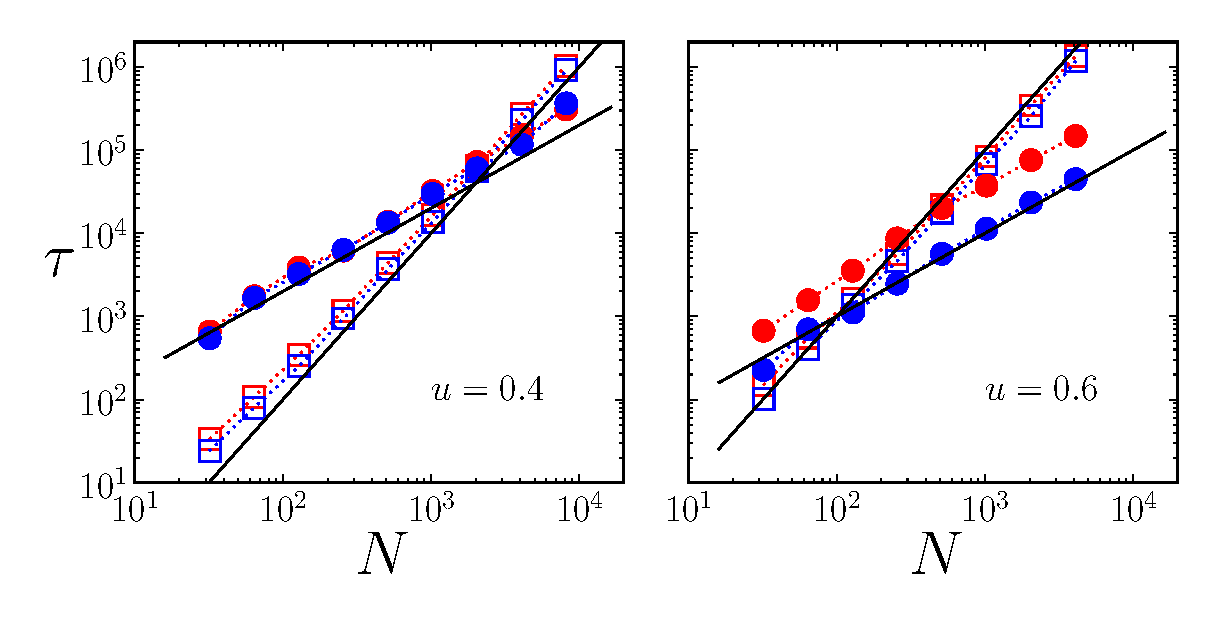
\includegraphics[width=1.0\linewidth]{./PlotTaus1over3_XY_HMF.pdf}
 \caption{$\tau$ vs $N$ for the short (square) and long (circle) range XY rotators, 
with energy densities $u=0.4$ (left) and $u=0.6$ (right). 
The red and blue symbols are for the hot and cold subsystems respectively. 
The black  solid line  $\tau \sim N$ and $N^2$ are drawn for comparison.}
 \label{fig:Taus_XY_HMF}
\end{figure}



\section{TO ADD IN THE BODY Spread of a perturbation in the ring}

In order to analyze the spread of the energy in the systems 
(\ref{eq:Potentials}), we apply a kinetic perturbation to the two 
central particles of the system\footnote{Due to the periodic 
boundary conditions the central particles could be any contiguous particles.}.
This perturbation consists in change the kinetic energy of the 
two central particles to the twice the value 
of the equilibrium kinetic energy, in opposite directions. 
Then the momentums of the rest of the particles are 
corrected to preserve the kinetic energy and 
total momentum of all the system.



\begin{figure}
 \centering
 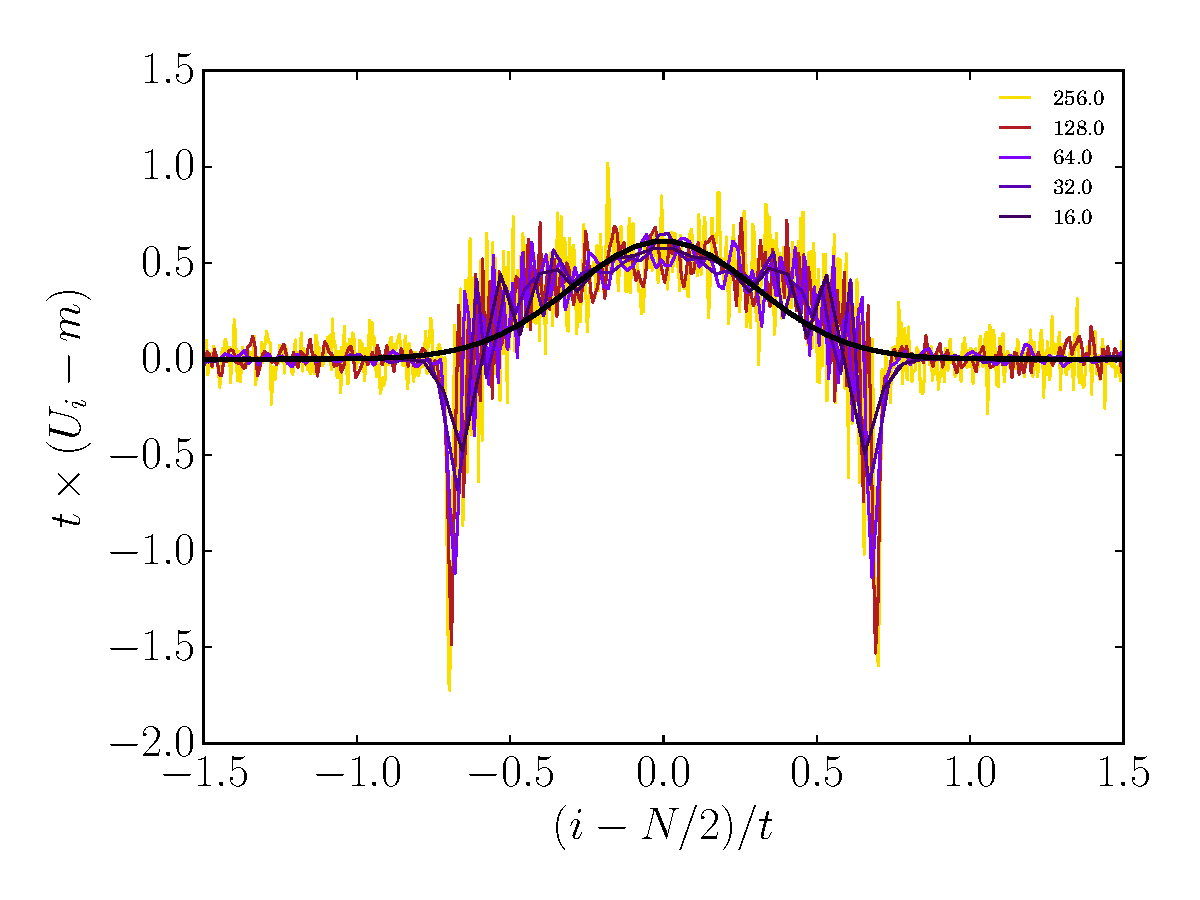
\includegraphics[width=1.0\linewidth]{./Time_NrgProf_HC__U0_0.4__N_1024.pdf}
 % Time_NrgProf_HC__U0_0.4__N_1024.pdf: 0x0 pixel, 300dpi, 0.00x0.00 cm, bb=
 \caption{Time scaled evolution of the energy profile (kinetic and potential) 
 under a perturbation in the middle of the ring, for harmonic potential (HC)
 with $u=0.4$ and $N=1024$. The black line is a fitted Gaussian curve and $m$ 
 is the mean energy of 20 particles at the other side of the ring.}
 \label{fig:Time_NrgProf_HC}
\end{figure}


\begin{figure}
 \centering
 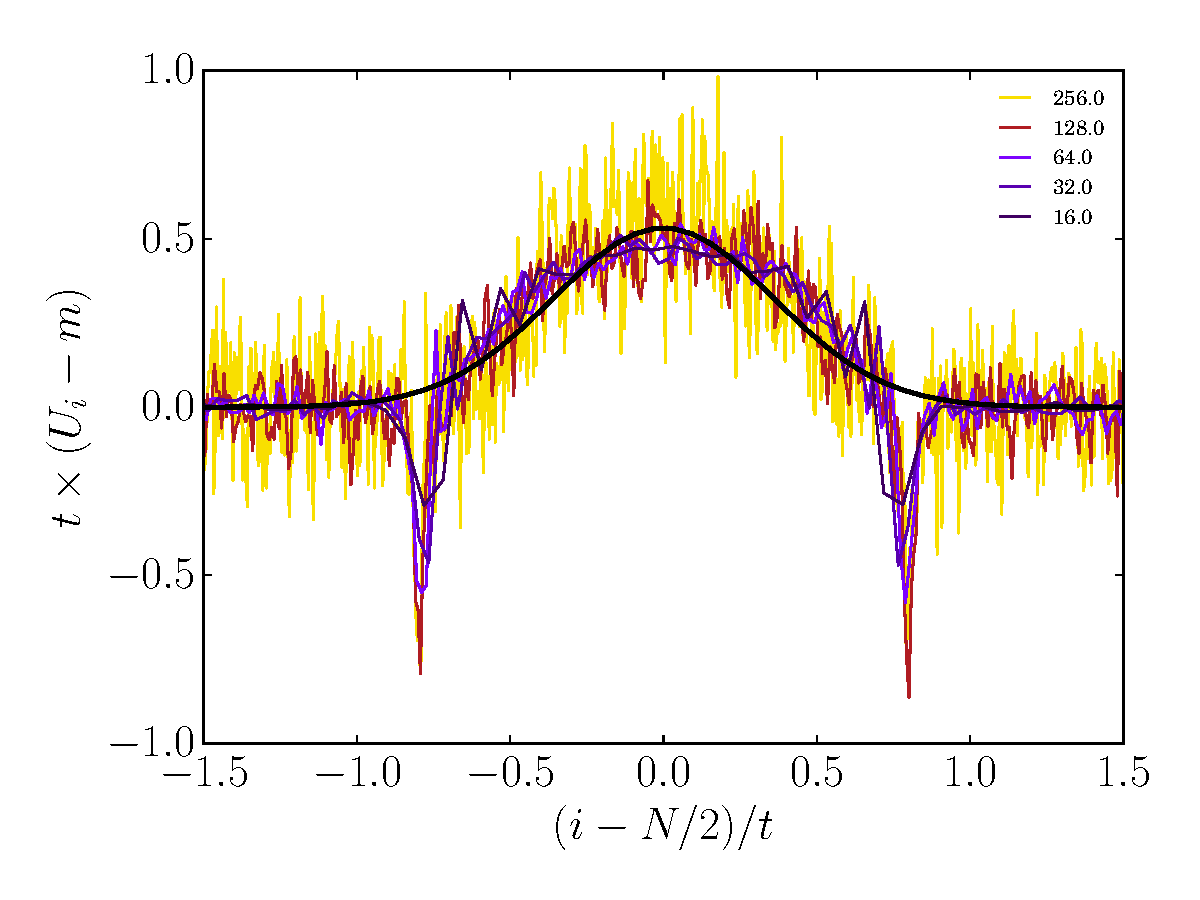
\includegraphics[width=1.0\linewidth]{./Time_NrgProf_FPU__U0_0.4__N_1024.pdf}
 % Time_NrgProf_HC__U0_0.4__N_1024.pdf: 0x0 pixel, 300dpi, 0.00x0.00 cm, bb=
 \caption{Time scaled evolution of the energy profile (kinetic and potential) 
 under a perturbation in the middle of the ring, for the FPUT-$\beta$ system
 with $u=0.4$ and $N=1024$. The black line is a fitted Gaussian curve and $m$ 
 is the mean energy of 20 particles at the other side of the ring.}
 \label{fig:Time_NrgProf_HC}
\end{figure}


\begin{figure}
 \centering
 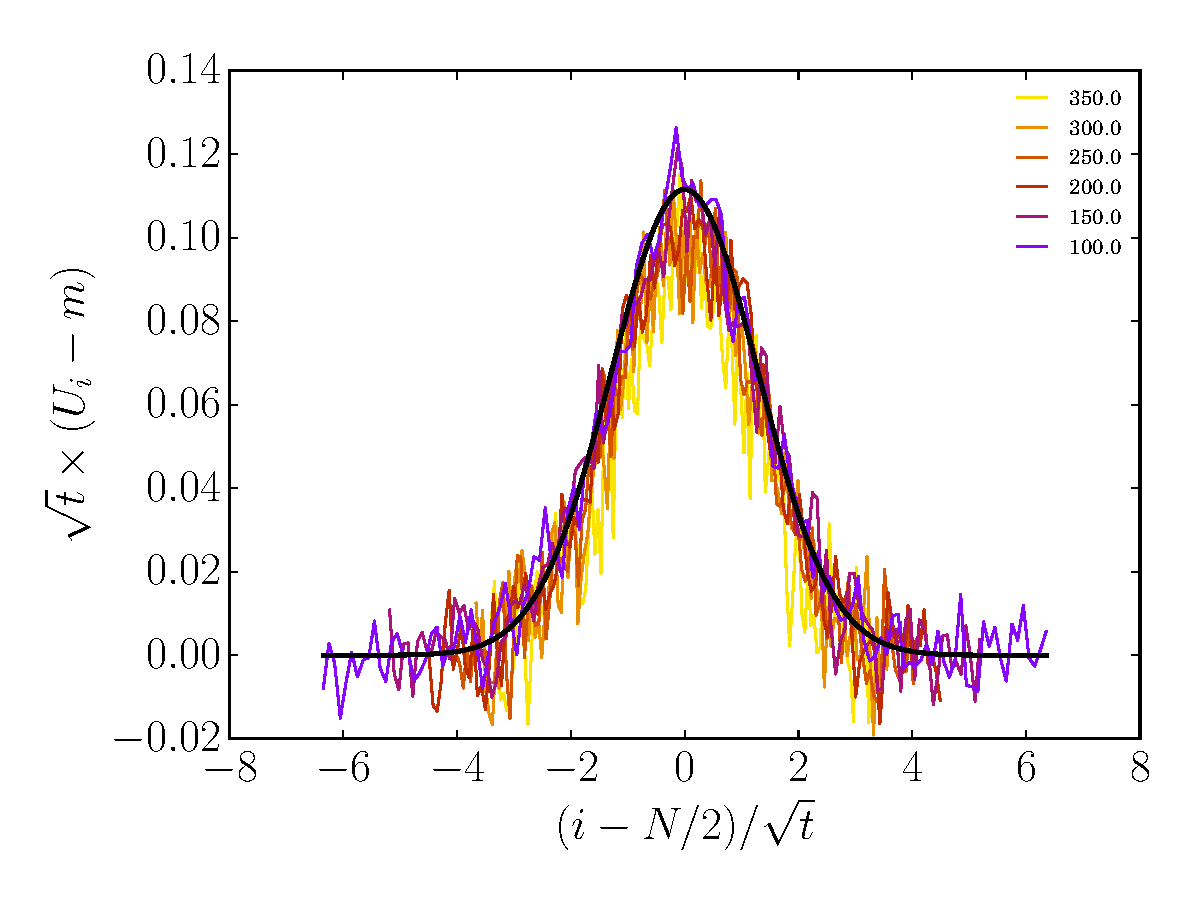
\includegraphics[width=1.0\linewidth]{./Time_NrgProf_XY__U0_0.4__N_128.pdf}
 % Time_NrgProf_HC__U0_0.4__N_1024.pdf: 0x0 pixel, 300dpi, 0.00x0.00 cm, bb=
 \caption{Time scaled evolution of the energy profile (kinetic and potential) 
 under a perturbation in the middle of the ring, for the XY system 
 with $u=0.4$ and $N=128$. The black line is a fitted Gaussian curve and $m$ 
 is the mean energy of 20 particles at the other side of the ring.}
 \label{fig:Time_NrgProf_HC}
\end{figure}




{\bf Acknowledgments:}
We thank Brazilian agencies CNPq and Faperj for partial financial support. 

%\newpage
%\bibliographystyle{apsrev4-1}
%\bibliography{longrange-cond-v1}

\bibliographystyle{apsrev4-1} %unsrt
\bibliography{Relax2EqRef}{}


% \begin{thebibliography}{99}
% 
% \bibitem{LepriBook2016}
% S. Lepri, R. Livi, A. Politi in  
% %\newblock {mensions: Introduction and phenomenology,” 
% {\em Thermal Transport in Low Dimensions: From Statistical Physics to Nanoscale Heat Transfer} Chap. 1, 
% S. Lepri, editor (Springer International Publishing, 2016).
% %
% 
% \end{thebibliography}
 
 
 
\end{document}         

